\documentclass[12pt]{report}
\usepackage[utf8]{inputenc}
\usepackage{polski}
\usepackage[polish]{babel}
\usepackage{graphicx}
\usepackage{adjustbox}
\usepackage{hyperref}
\usepackage{float}
\usepackage{listings}
\graphicspath{ {images/} }
\usepackage{color}


\definecolor{mygreen}{rgb}{0,0.6,0}
\definecolor{mygray}{rgb}{0.5,0.5,0.5}
\definecolor{mymauve}{rgb}{0.58,0,0.82}

\lstset{
  showstringspaces=false,
  frame={top, bottom},
  backgroundcolor=\color{white},   % choose the background color
  basicstyle=\footnotesize,        % size of fonts used for the code
  captionpos=b,                    % sets the caption-position to bottom
  commentstyle=\color{mygreen},    % comment style
  keywordstyle=\color{blue},       % keyword style
  stringstyle=\color{mymauve}     % string literal style
}


\title{
        {Zastosowania systemów wbudowanych}\\
        {
\includegraphics{pwr.png}}
}

\author{
Miłosz Białczak\\
Mateusz Gniewkowski\\
Beata Szeląg\\[15pt]
Prowadzący: dr inż. Marek Woda
}

\date{DD:MM:RR}

\begin{document}

\maketitle

\tableofcontents

%\chapter{chapt}
%\input{chapters/chapt}

\chapter{Wstęp}
Nowoczesne rozwiązania technologiczne pozwalają domowym użytkownikom na budowę systemów wbudowanych dostosowanych do ich potrzeb. Platformy takie jak \emph{Raspberry PI} czy \emph{Arduino}, w połączeniu z wieloma czujnikami dostępnymi na rynku, dają możliwości, które jeszcze kilka lat temu były niewyobrażalne. Projekt, którego dotyczy niniejsza dokumentacja, jest przykładem systemu, który został zrealizowany właśnie dzięki tego typu rozwiązaniom. Będzie on umożliwiał rozmowę ze sztuczną inteligencją udostępnianą przez \emph{Google} (\emph{Google Assistant}). Pozwala ona między innymi na sprawdzenie pogody, swojej skrzynki mailowej, kalendarza i innych usług udostępnianych przez \emph{Google}. Oprócz tego możemy zadać jej właściwe każde pytanie.


System zostanie rozbudowany o możliwość sprawdzenia stanu fizycznej skrzynki pocztowej. Ma ono następować poprzez stronę internetową lub komendę głosową, na którą urządzenie odpowie nam odpowiednim komunikatem. W tym celu zostanie stworzony serwer aplikacji, serwer webowy oraz osobny podsystem oparty na module \emph{ESP8266} pozwalający na zbadanie aktualnego stanu skrzynki. Komunikacja urządzeń będzie wymagała sieci WiFi oraz dostępu do Internetu.

Ten dokument składa się z sześciu rozdziałów. Pierwszy z nich stanowi niniejszy wstęp. W drugim zostaną omówione założenia projektowe. W trzecim można znaleźć informacje o wykorzystanych technologiach. W czwartym zostanie opisany projekt poszczególnych elementów systemu. W piątym znajdą się szczegółowe informacje dotyczące realizacji części projektowej. Ostatni rozdział zostanie poświęcony na uwagi i wnioski jakie wyniknęły podczas realizacji projektu.

\chapter{Założenia projektowe}
Poniżej przedstawiono listę wymagań systemu.


\begin{enumerate}

\item System musi pozwalać na werbalną komunikację z \emph{Google Assistant}.
\item System musi pozwalać na sprawdzenie stanu fizycznej skrzynki pocztowej w sposób werbalny i poprzez stronę internetową.
\item Podsystem oparty na \emph{ESP8266} musi mieć możliwość działania na bateryjnym źródle zasilania.
\item Podsystem oparty na \emph{ESP8266} musi w sposób rozsądny korzystać ze źródła zasilania.
\item Podsystem oparty na \emph{ESP8266} powinien dawać możliwość ustalenia czasu, w którym dostaliśmy listy.
\item System powinien umożliwiać implementowanie własnych komend.
\item System powinien umożliwiać odtwarzanie muzyki z portalu \emph{YouTube}.

\end{enumerate}

\chapter{Technologie}
Niżej została przedstawiona lista technologii, które zostaną wykorzystane w systemie. System będzie zbudowany z dwóch urządzeń - \emph{Raspberry Pi} i \emph{ESP8266} oraz szeregu peryferiów do nich podłączonych (ich dokładną listę można znaleźć w kolejnym podrozdziale).

\begin{enumerate}

\item \textbf{Python} - zarówno serwer jak i aplikacja komunikująca się z \emph{Google Assistant} zostanie napisane w języku \emph{Python}

\item \textbf{Flask} - \emph{Flask} jest framework'iem pozwalającym na budowę serwerów aplikacji typu \emph{REST}

\item \textbf{C++} - do zaprogramowania modułu \emph{ESP8266} zostanie użyty język \emph{C++}

\item \textbf{HTML5 + CSS + JS + AngularJS} - niniejsze technologie zostaną wykorzystane do napisania aplikacji webowej. 



\end{enumerate}

\chapter{Projekt Systemu}
\section{Projekt systemu}
\begin{center}
	\label{img:system}
	\adjustbox{valign=t}{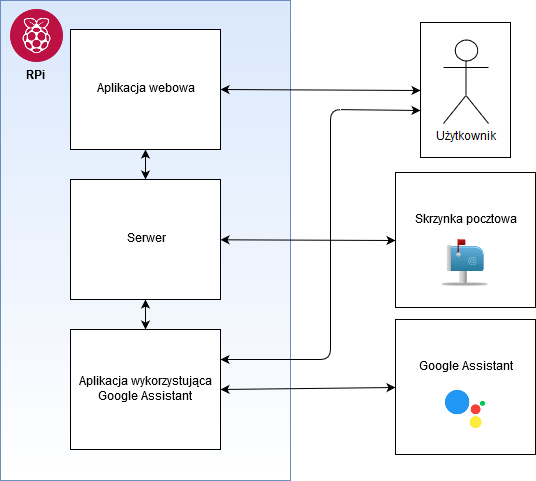
\includegraphics[width=12cm]{schemat.png}}
\end{center}
Rysunek \ref{img:system} przedstawia ogólny schemat opisywanego projektu.
Jego kolejne części są opisane w poniższych sekcjach:
\begin{itemize}
\item część RPI + Google Assistant w sekcji \textit{Raspberry Pi - Google Assistant}
\item część z ESP8266 w sekcji \textit{ESP8266}
\item serwer w sekcji \textit{Serwer}
\item aplikacja webowa w sekcji \textit{Aplikacja webowa}
\end{itemize}


\section{Raspberry Pi - Google Assistant}

Głównym elementem naszego projektu jest mikrokomputer Raspberry Pi 3 w wersji B. Zostanie na nim zainstalowany serwer aplikacji webowej (omówiony w rozdziale <tu wstaw rozdział> i Google Assistant. W niniejszej części dokumentu zostanie omówiony projekt bezpośredniego połączenia Raspberry Pi z urządzeniami zewnętrznymi (takimi jak głośnik, mikrofon) stanowiącymi razem pewną integralną całość, w założeniu mającą znaleźć się w jednej obudowie. Zdalny moduł wykorzystujący ESP8266 zostanie omówiony w innej części tego dokumentu.

\begin{center}
	\label{img:google}
	\adjustbox{valign=t}{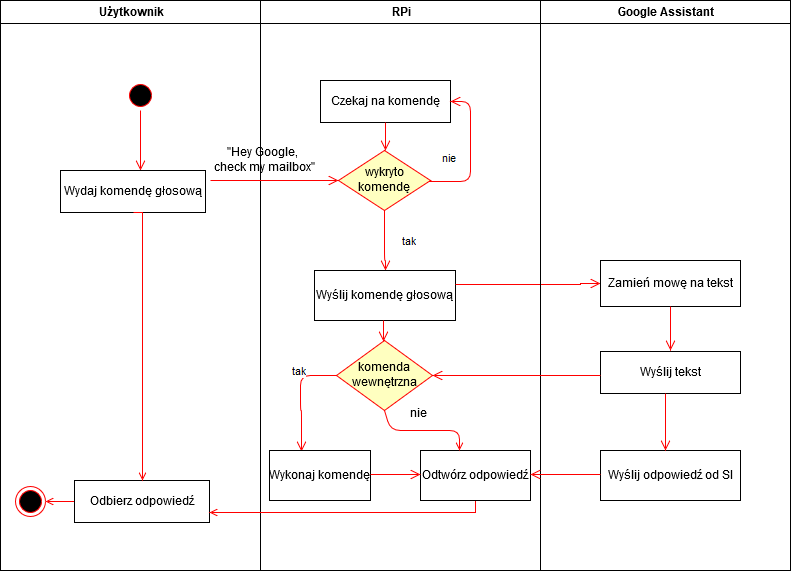
\includegraphics[width=14cm]{google.png}}
\end{center}
Rysunek \ref{img:google} przedstawia schemat części opartej o RPI i Google Assistanta.

\subsection{Spis urządzeń}

	\begin{figure}[H]
	\centering
	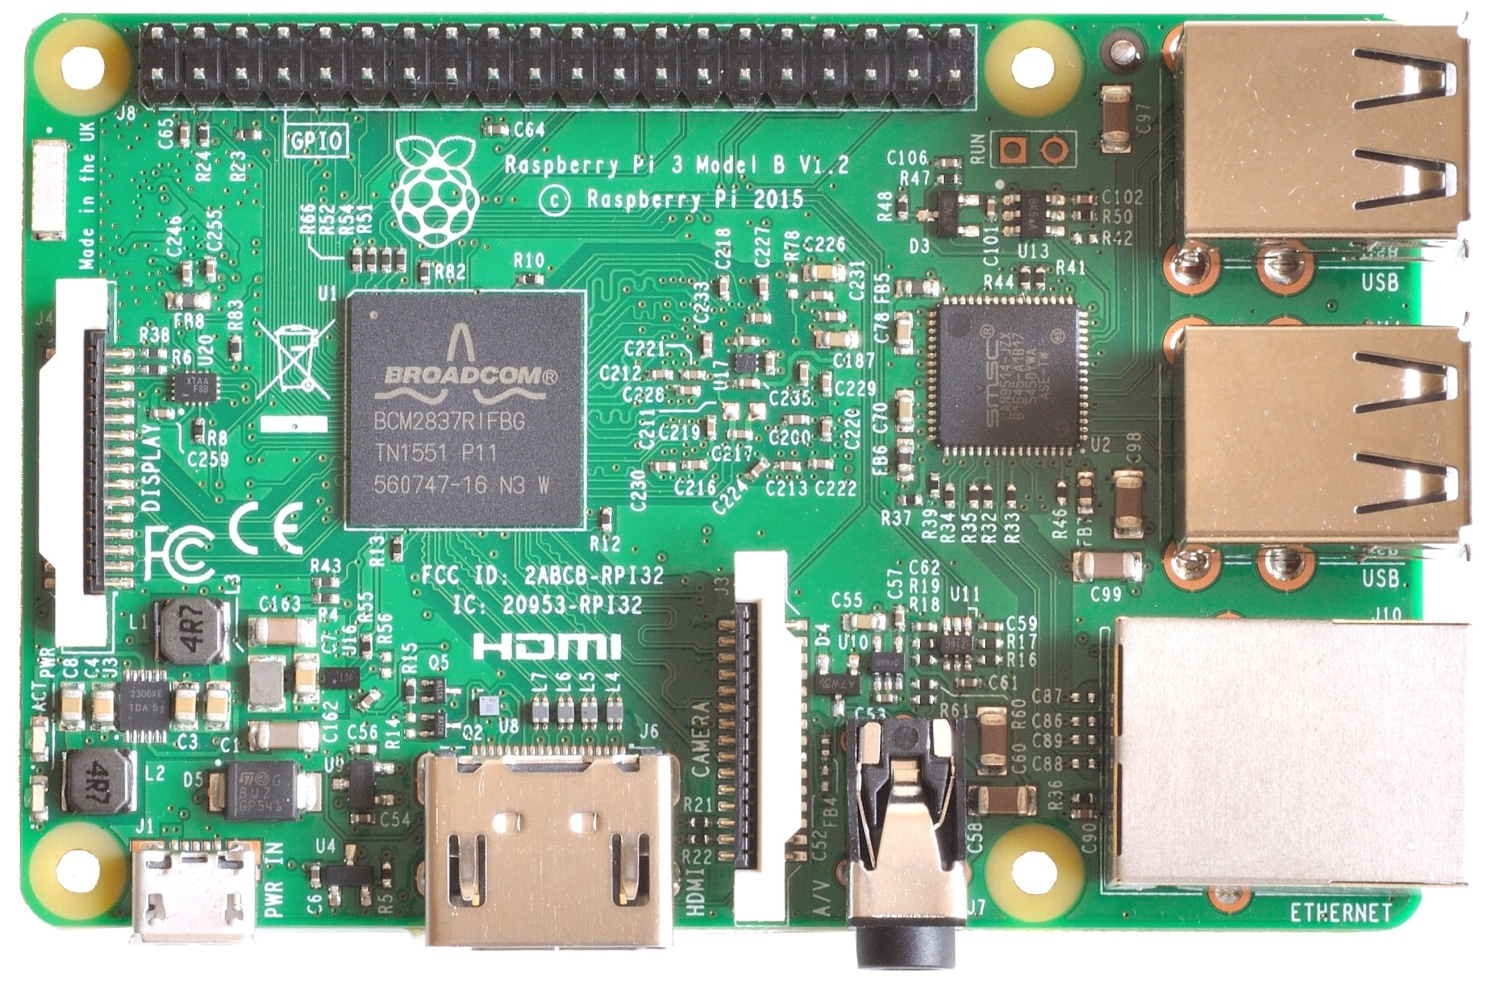
\includegraphics[width=8cm]{rpi.jpg}
	\caption{Raspberry Pi 3 w wersji B}
	\end{figure}
	
	\begin{figure}[H]
	\centering
	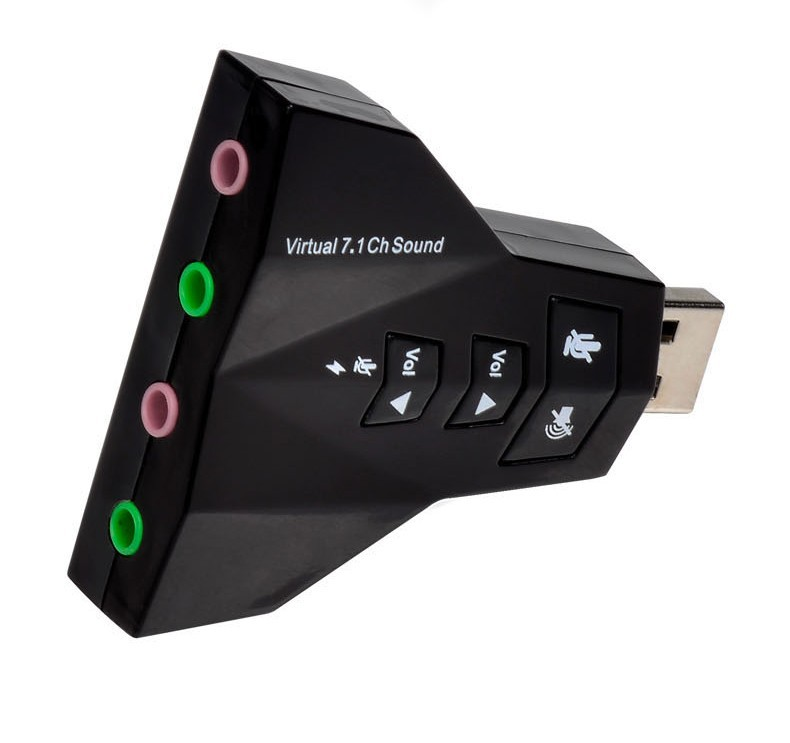
\includegraphics[width=8cm]{karta_muzyczna.jpg}
	\caption{Zewnętrzna karta dżwiękowa Virtual 7.1 Channel USB }
	\end{figure}
	
	\begin{figure}[H]
	\centering
	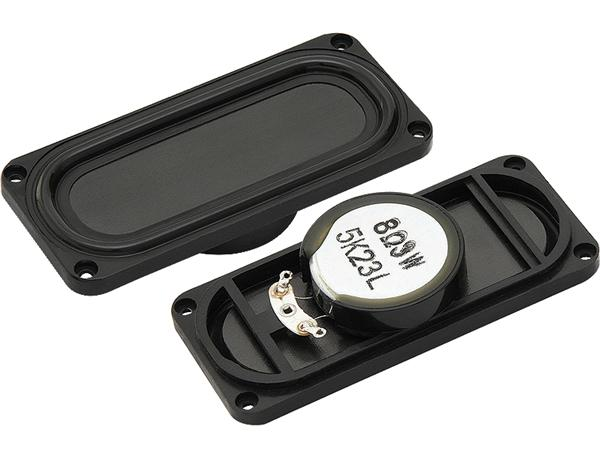
\includegraphics[width=8cm]{glosnik.jpg}
	\caption{Głośnik 3W 8Ohm 40x88mm}
	\end{figure}
	
	\begin{figure}[H]
	\centering
	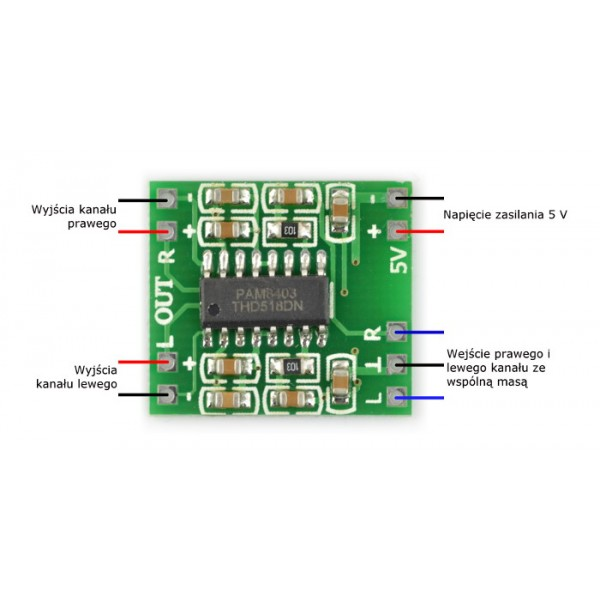
\includegraphics[width=8cm]{wzmacniacz.jpg}
	\caption{Wzmacniacz audio stereo PAM8403 5V 3W - dwukanałowy}
	\end{figure}
	
	\begin{figure}[H]
	\centering
	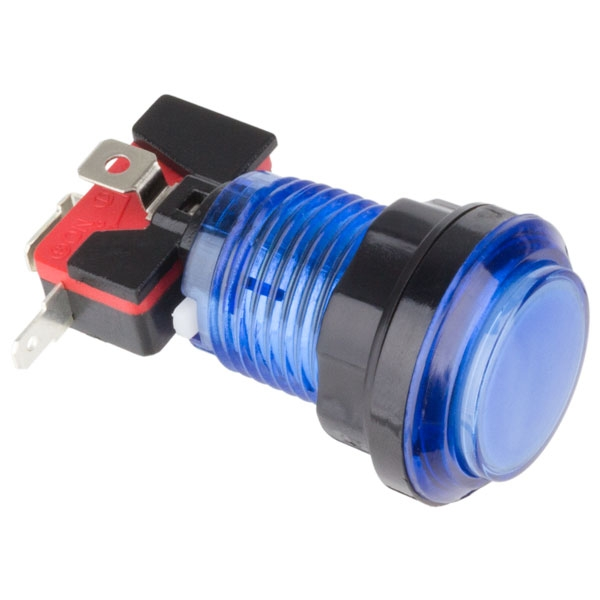
\includegraphics[width=8cm]{button.jpg}
	\caption{Rrzycisk Arcade Push Button niebieski z podświetleniem}
	\end{figure}

Dodatkowo zostanie wykorzystany mikrofon wykorzystujący złącze typu \emph{mini jack}.

\subsection{Schemat połączeń}

Na poniższym schemacie zaprezentowano układ połączeń wyżej wymienionych elementów. Rezystancje oporników mogą się różnić ze względu na wykorzystany tranzystor i rodzaj diody świecącej. W większości przypadków układ typu "klucz npn" nie będzie potrzebny, gdyż napięcie przewodzenia diody może okazać na tyle niskie, że będzie możliwe zasilenie jej z portu GPIO (niestety nie było tak w naszym przypadku).

\begin{center}
\adjustbox{valign=t}{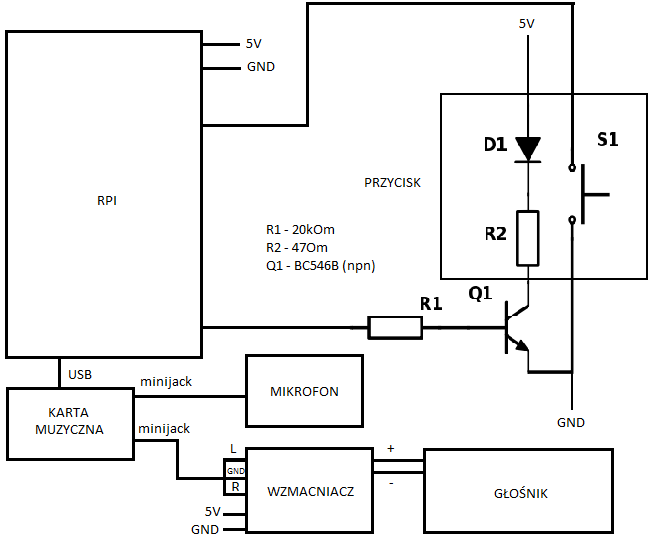
\includegraphics[width=8cm]{schematRPI.png}}
\end{center}


\section{ESP8266}

Drugim kluczowym elementem naszego projektu jest układ wykorzystujący moduł \emph{ESP8266}. Zostanie do niego podłączony nadajnik IR, odbiornik IR i bateria. Gdy odczyt sygnału, nadawanego przez pierwsze z urządzeń, nie będzie możliwy, znaczy to, że na drodze wiązki znajduje się jakaś przeszkoda - w założeniach ma to być list. Moduł zostanie oprogramowany tak aby, co jakiś ustalony czas, wysyłać do serwera informacje o odczycie. W finalnej wersji układ ma zostać zamontowany w skrzynce.
\subsection{Spis urządzeń}



	\begin{figure}[H]
	\centering
	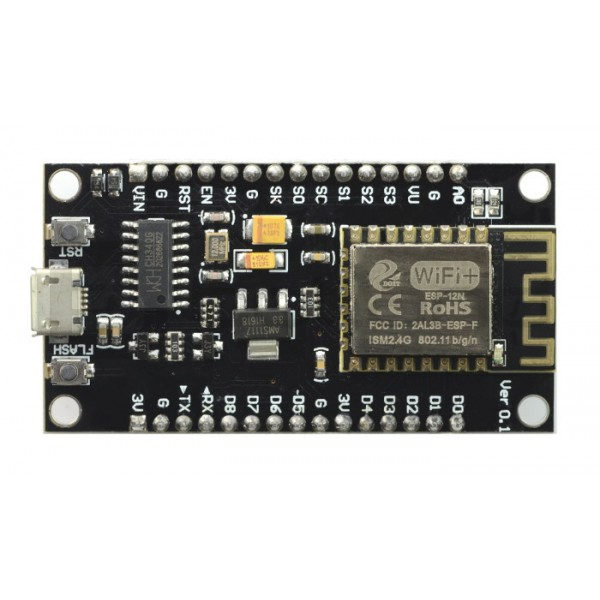
\includegraphics[width=7cm]{esp8266-nodemcu-v3.jpg}
	\caption{ESP8266 z ModeMCU v3}
	\end{figure}
	
	\begin{figure}[H]
	\centering
	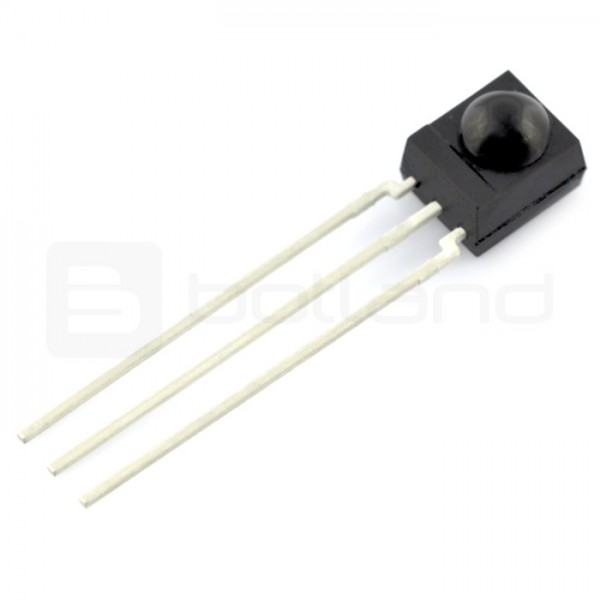
\includegraphics[width=7cm]{tsop4836.jpg}
	\caption{Odbiornik TSOP4836 }
	\end{figure}
	
	
	\begin{figure}[H]
	\centering
	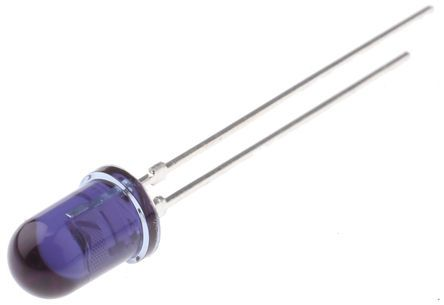
\includegraphics[width=7cm]{LIRED5C.jpg}
	\caption{Nadajnik IR LIRED5C}
	\end{figure}

\subsection{Schemat połączeń}

Poniższy schemat przedstawia układ połączeń wyżej wymienionych elementów. Warto zwrócić uwagę na połączenie pinu GPIO\_16 z pinem REST. Pozwoli to przełączać moduł ESP w tryb głębokiego snu - pozwoli to na oszczędzanie baterii.

\begin{center}
	\adjustbox{valign=t}{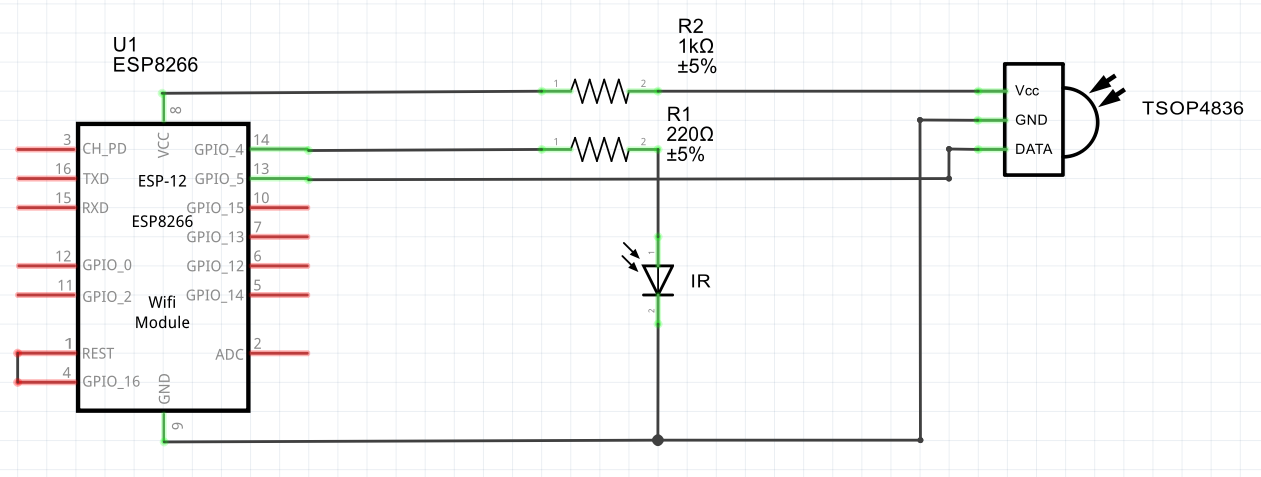
\includegraphics[width=8cm]{schematWiFI_IR.png}}
\end{center}

\section{Serwer}

Następną częścią projektu jest serwer oparty o technologię \textit{Flask}. Pozwala on na komunikację pomiędzy \textit{ESP8266}, \textit{Google Assistantem} oraz aplikacją webową.\\

Serwer jest uruchamiany na \textit{Raspberry PI}, na porcie 5000 i udostępnia klientom dwa \textit{endpointy}. Jeden z nich pozwala na pobranie aktualnego stanu skrzynki pocztowej, drugi - na jego zmianę. \\

REST API udostępniane przez serwer jest przedstawione w tabeli \ref{tab:api}.

\begin{longtable}{|c|c|c|p{4cm}|}
\caption{Serwer REST API} \label{tab:api} \\ \hline
\multicolumn{4}{ |c| }{ Skrzynka pocztowa } \\ \hline
\multicolumn{4}{ |c| }{ /state } \\ \hline
Endpoint & Request & Opis & Dodatkowo \\ \hline
/state & GET & Pobranie informacji o stanie skrzynki & Rezultat: 0 - pusta skrzynka, 1 - pełna \\ \hline
/state/[state] & POST & Zmiana stanu na [state] & state może przyjąć wartości: 0 lub 1 \\ \hline
\end{longtable} 

\begin{center}
	\label{img:serwer_class}
	\adjustbox{valign=t}{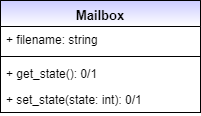
\includegraphics[width=6cm]{serwer_class.png}}
\end{center}

Serwer korzysta z klasy Mailbox, która udostępnia dwie metody: do pobrania stanu skrzynki i do ustawienia stanu skrzynki. Więc o obu metodach można znaleźć w rozdziale 5 \textit{Realizacja}. Diagram klasy jest widoczny na rysunku \ref{img:serwer_class}

Stan skrzynki jest zapisywany w pliku, w postaci:
\begin{itemize}
\item 0 - gdy skrzynka jest pusta
\item 1 - gdy w skrzynce mamy jakieś wiadomości
\end{itemize}

W przypadku, jeśli na \textit{Raspberry PI} nie ma wymaganych przez serwer zależności (Flask w wersji 0.10.1) należy wywołać:
\begin{lstlisting}
pip install -r requirements.txt
\end{lstlisting}

Uruchamianie serwera następuje przez wywołanie:
\begin{lstlisting}
python run.py
\end{lstlisting}


\section{Aplikacja webowa}

\begin{center}
	\label{img:skrzynka}
	\adjustbox{valign=t}{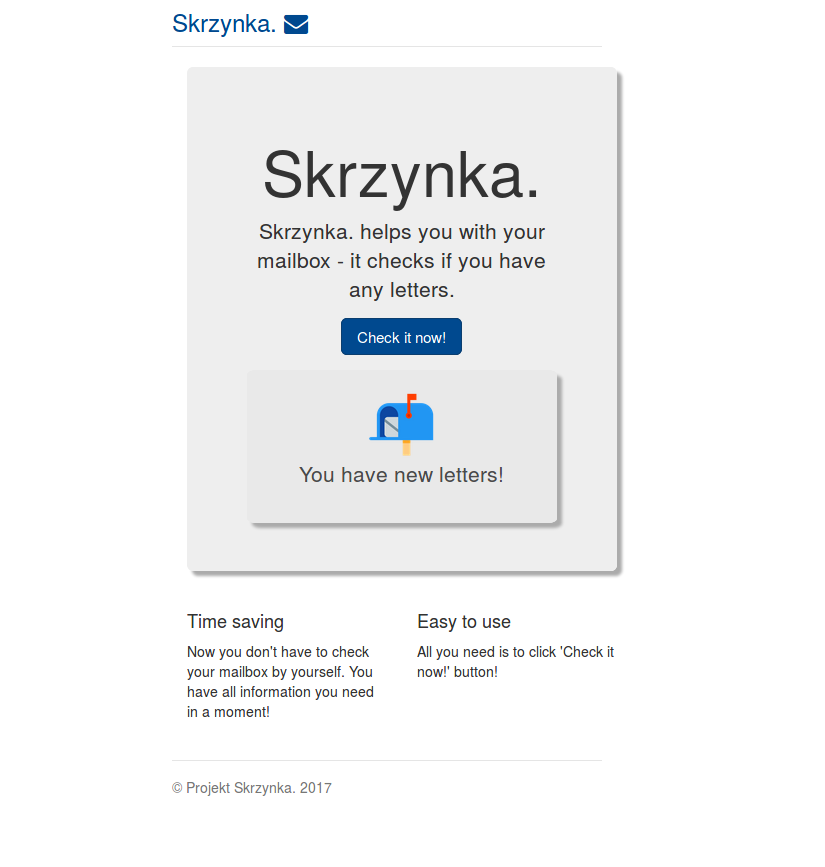
\includegraphics[width=10cm]{skrzynka2.png}}
\end{center}

Aplikacja webowa pozwala na sprawdzenie aktualnego stanu skrzynki pocztowej. Jest widoczna na rysunkach \ref{img:skrzynka}.
Logika aplikacji została stworzona w języku \textit{Java Script} wraz z \textit{AngularJS}, natomiast widok to \textit{HTML5} wraz z arkuszami stylów (\textit{CSS}).\\

Składa się z trzech głównych części:
\begin{itemize}
\item widoku - który określa elementy, jakie są obecne na stronie
\item kontrolera - który odpowiada za logikę w aplikacji (wykorzystuje serwis do wysyłania zapytań do serwera)
\item serwisu - który wysyła zapytanie \textbf{GET /state} na adres serwera
\end{itemize}

Na stronie dostępny jest przycisk \textbf{Check it now!} (ang. \textit{Wypróbuj już teraz!}), który wywołuje metodę kontrolera odpowiedzialną za wykonanie zapytania do serwera przez serwis.

\begin{center}
	\label{img:web_diagram}
	\adjustbox{valign=t}{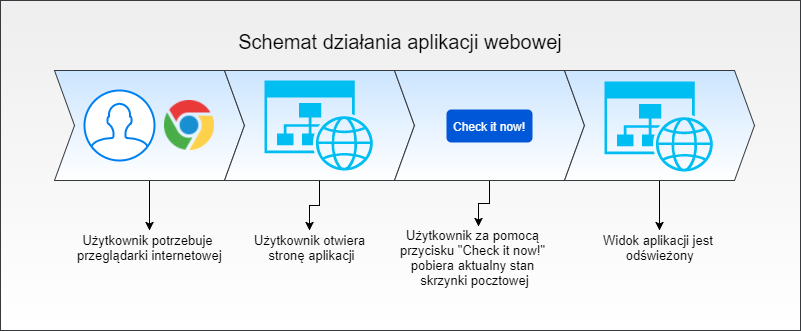
\includegraphics[width=14cm]{web_diagram.png}}
\end{center}

Rysunek przedstawiony wyżej (\textit{Schemat działania aplikacji webowej}) przedstawia schemat działania aplikacji webowej.

Uruchomienie serwera \textit{node.js} z parametrem wskazującym na ścieżkę do pliku \textbf{server.js}:
\begin{lstlisting}
node server.js
\end{lstlisting}

W przypadku, jeśli na \textit{Raspberry PI} nie ma wymaganych przez aplikację zależności należy wywołać:
\begin{lstlisting}
bower install
npm install connect
npm install serve-static
\end{lstlisting}
i później uruchomić serwer \textit{node.js}.
%
%	\begin{figure}
%	\centering
%	\label{img:skrzynka2}
%	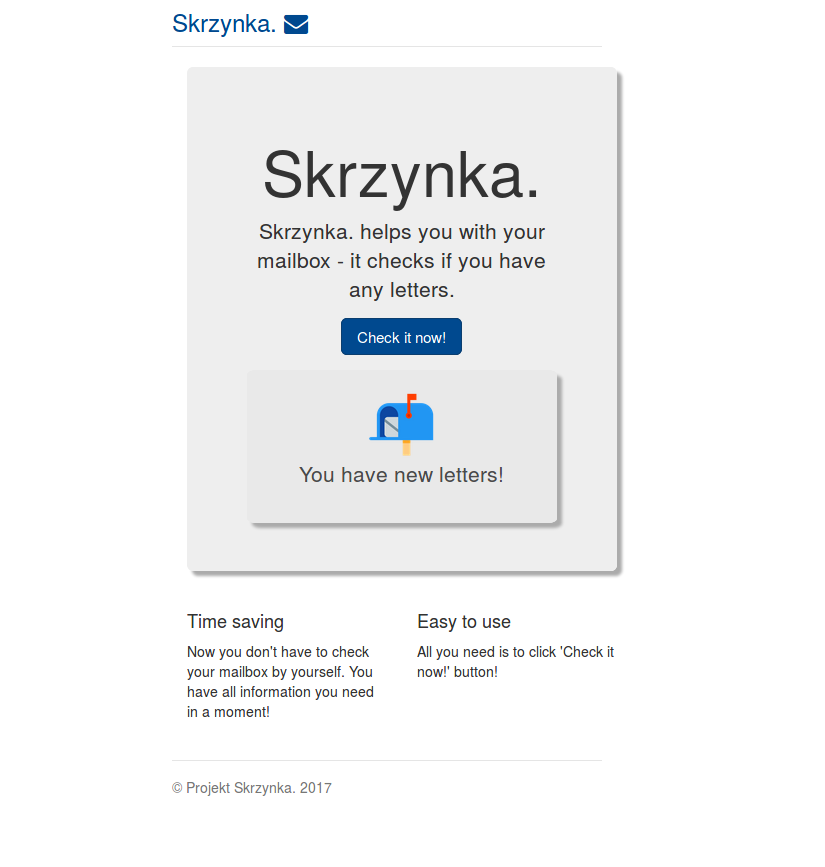
\includegraphics[width=10cm]{skrzynka2.png}
%	\caption{skrzynka2}
%	\end{figure}



\chapter{Realizacja}
\section{Raspberry Pi - Google Assistant}

\subsection{Projekt fizyczny}

Na podstawie schematu (dostępnego w poprzednim rozdziale) został zbudowany prototyp urządzenia pełniącego rolę asystenta.

\begin{center}
\adjustbox{valign=t}{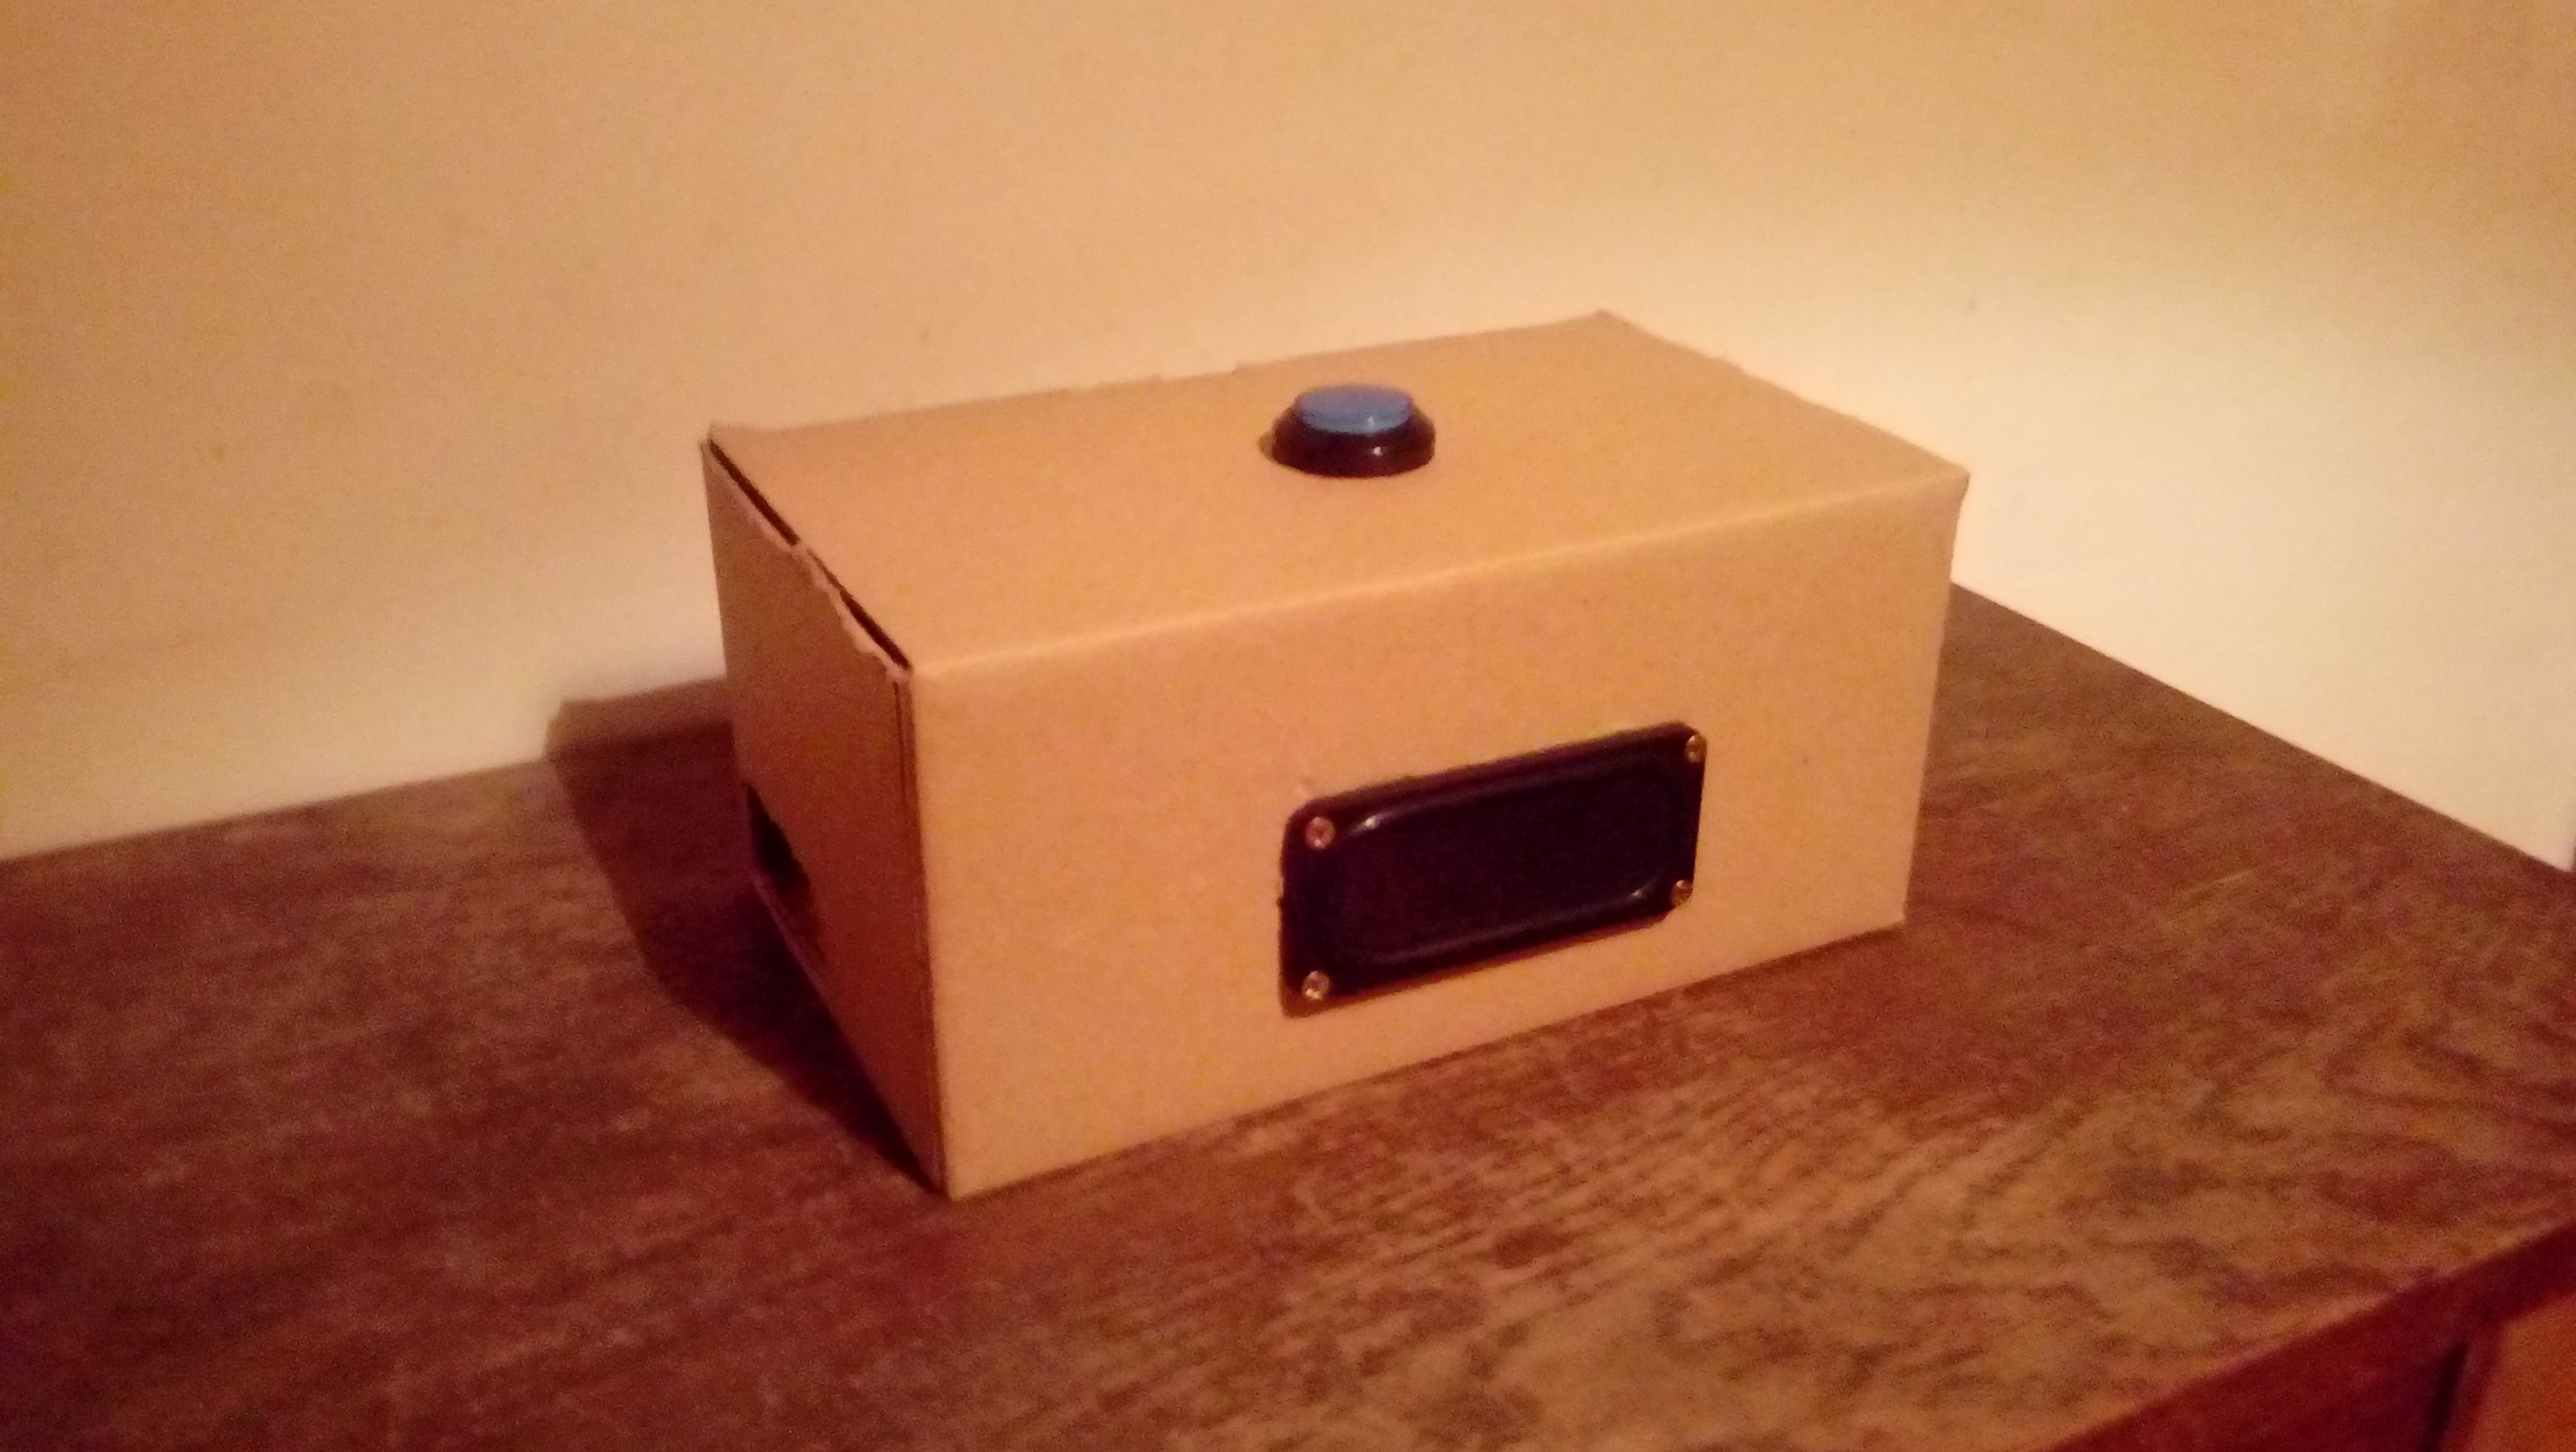
\includegraphics[width=10cm]{out.jpg}}
\end{center}
	
\begin{center}
\adjustbox{valign=t}{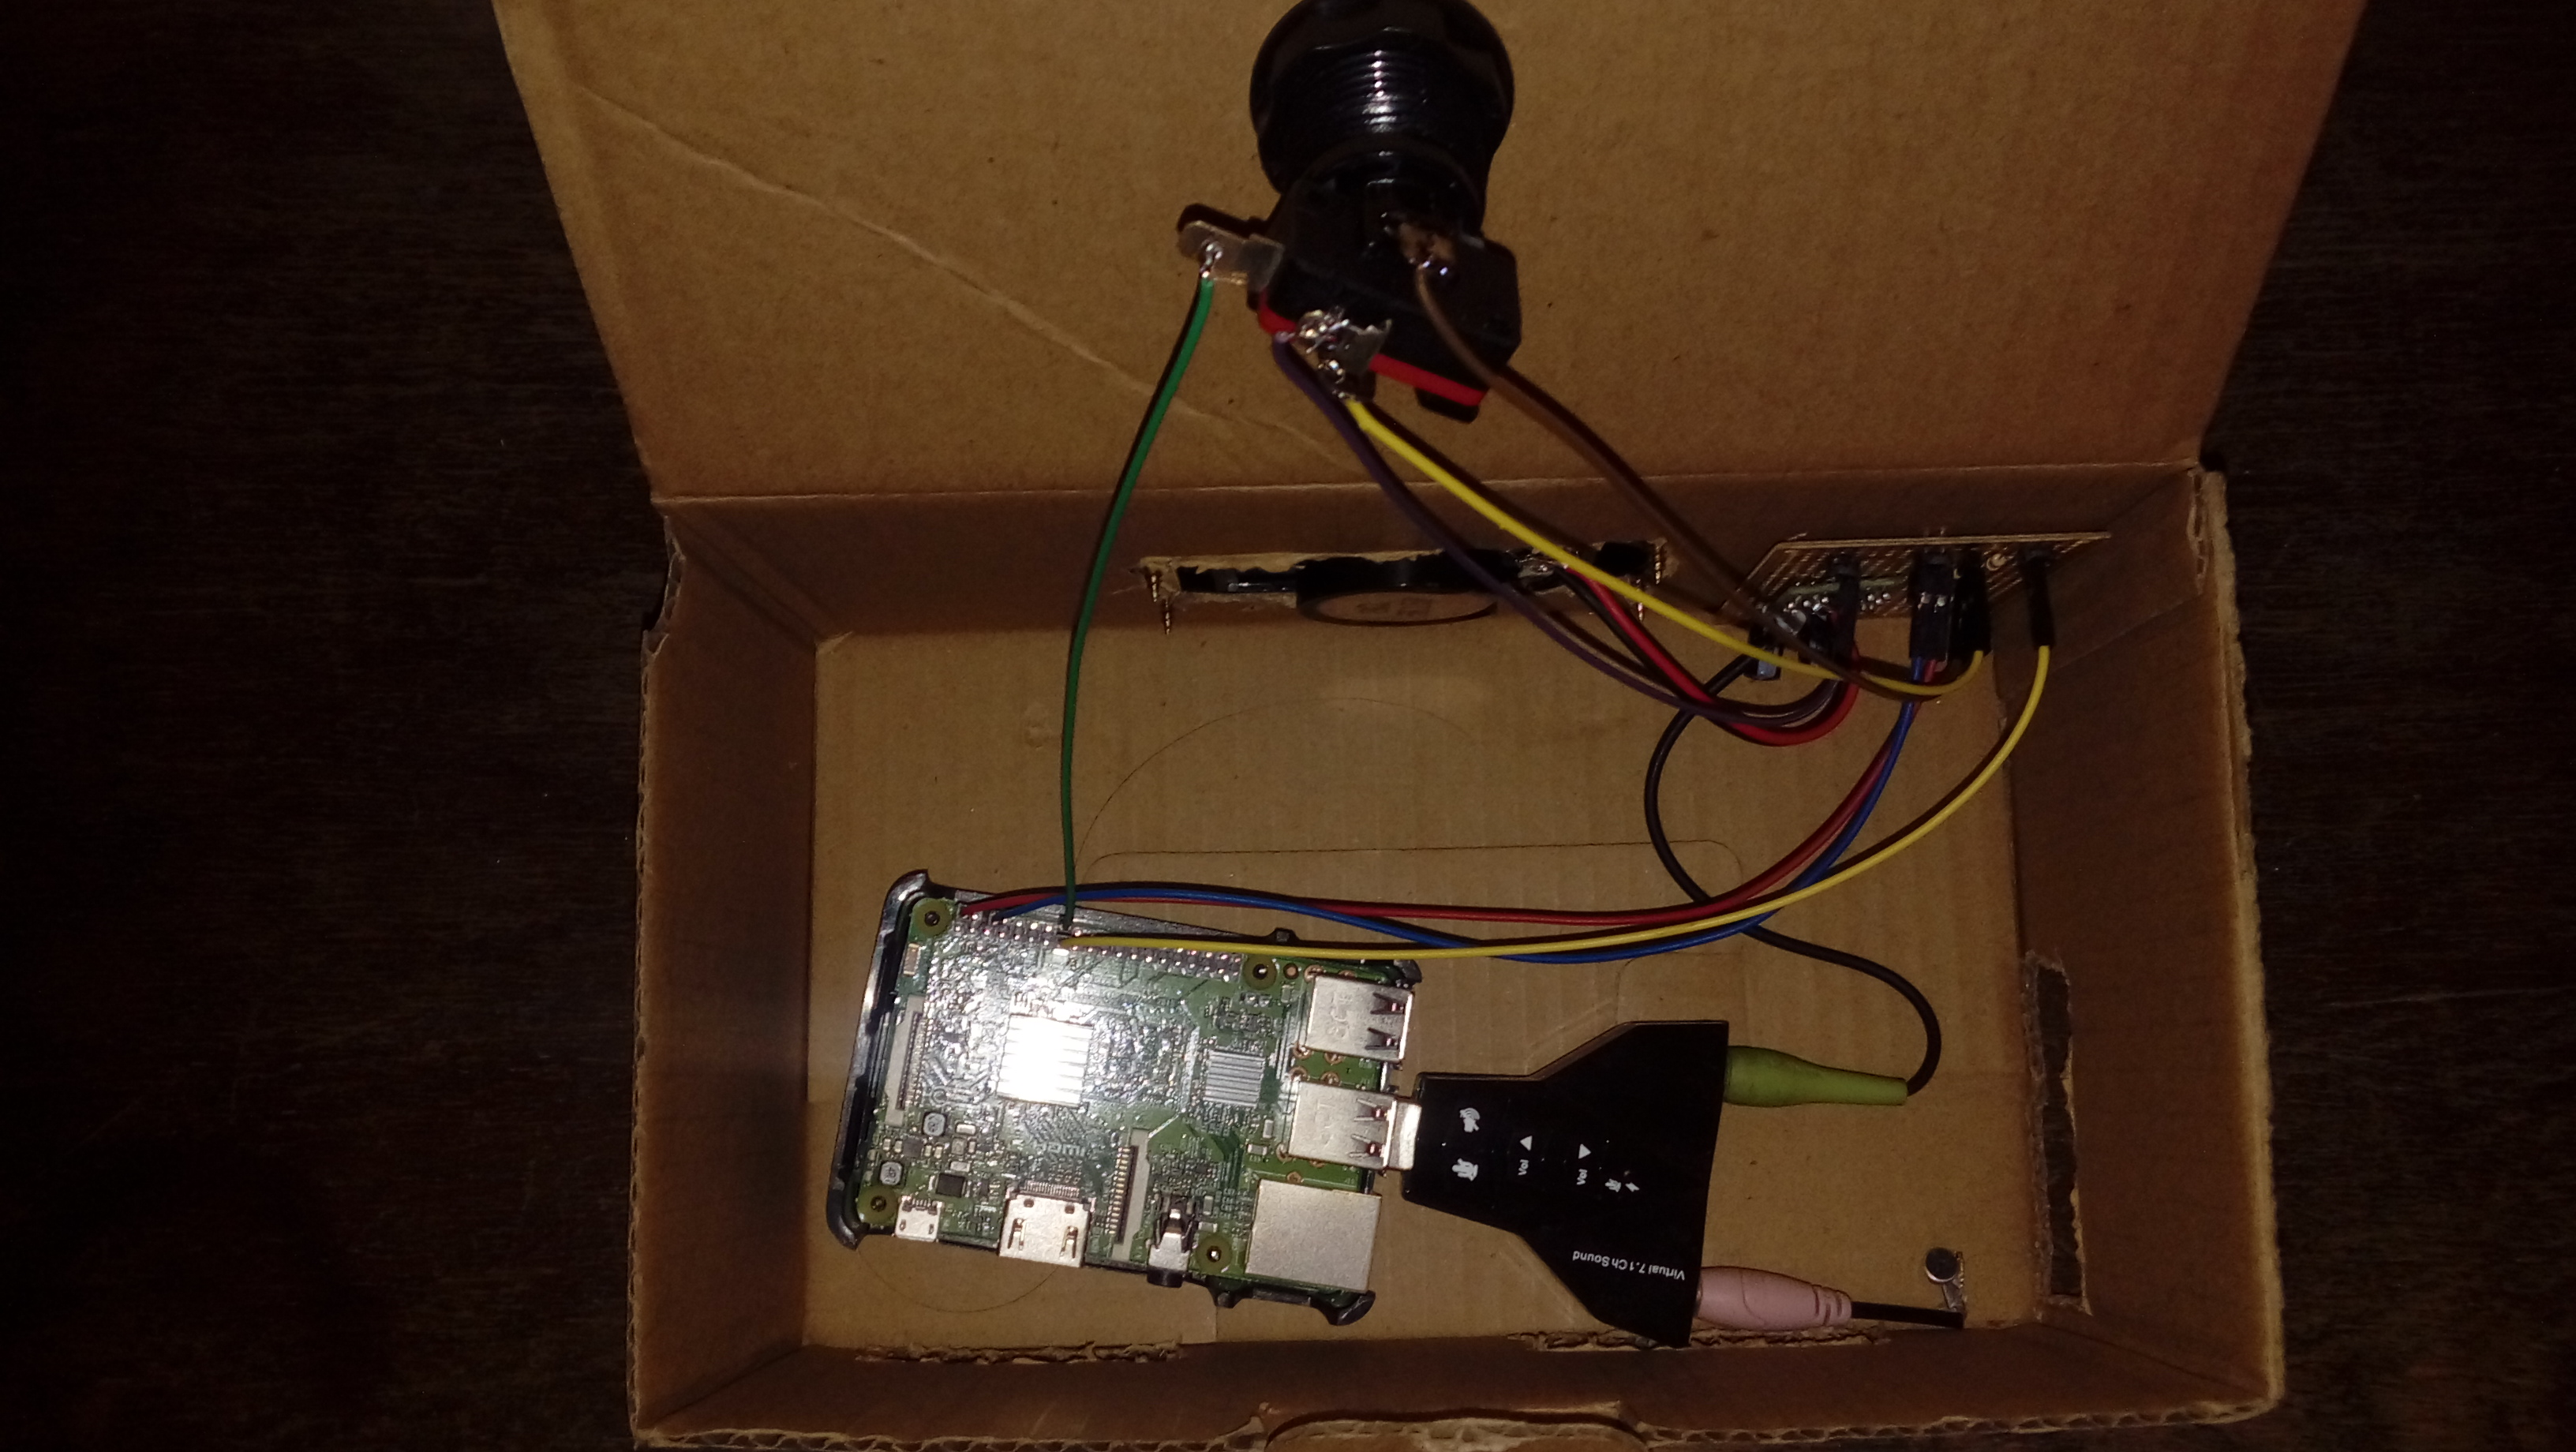
\includegraphics[width=10cm]{in.jpg}}
\end{center}

\subsection{Instalacja Google Assistant}

Podstawowa konfiguracja Google Assistant jest bardzo dobrze opisana na stronie \url{https://developers.google.com/assistant/sdk/overview} (zakładka ,,Python'').

\subsection{Opis pliku wejściowego}

Zakładając projekt z wykorzystujący Google Assistant SDK dostajemy skrypt realizujący podstawową funkcjonalność asystenta:


\begin{lstlisting}[language=Python]
#!/usr/bin/env python

# Copyright (C) 2017 Google Inc.
#
# Licensed under the Apache License, Version 2.0 (the 'License');
# you may not use this file except in compliance with the License.
# You may obtain a copy of the License at
#
#     http://www.apache.org/licenses/LICENSE-2.0
#
# Unless required by applicable law or agreed to in writing, software
# distributed under the License is distributed on an 'AS IS' BASIS,
# WITHOUT WARRANTIES OR CONDITIONS OF ANY KIND, either express or implied.
# See the License for the specific language governing permissions and
# limitations under the License.


from __future__ import print_function

import argparse
import os.path
import json

import google.oauth2.credentials

from google.assistant.library import Assistant
from google.assistant.library.event import EventType
from google.assistant.library.file_helpers import existing_file


def process_event(event):
    '''Pretty prints events.
    Prints all events that occur with two spaces between each new
    conversation and a single space between turns of a conversation.
    Args:
        event(event.Event): The current event to process.
    '''
    if event.type == EventType.ON_CONVERSATION_TURN_STARTED:
        print()

    print(event)

    if (event.type == EventType.ON_CONVERSATION_TURN_FINISHED and
            event.args and not event.args['with_follow_on_turn']):
        print()


def main():
    parser = argparse.ArgumentParser(
        formatter_class=argparse.RawTextHelpFormatter)
    parser.add_argument('--credentials', type=existing_file,
                        metavar='OAUTH2_CREDENTIALS_FILE',
                        default=os.path.join(
                            os.path.expanduser('~/.config'),
                            'google-oauthlib-tool',
                            'credentials.json'
                        ),
                        help='Path to store and read OAuth2 credentials')
    args = parser.parse_args()
    with open(args.credentials, 'r') as f:
        credentials = google.oauth2.credentials.Credentials(token=None,
                                                            **json.load(f))

    with Assistant(credentials) as assistant:
        for event in assistant.start():
            process_event(event)


if __name__ == '__main__':
    main()
    
\end{lstlisting}

Powyższy kod tworzy obiekt asystenta (wykorzystując w tym procesie dane uwierzytelniające),
po czym w pętli zaczyna przetwarzanie zdarzeń (przykładem zdarzenia jest początek konwersacji wywoływany słowami ,,Hey Google'').
Zmieniając implementację metody process\_event możemy wpływać na zachowanie asystenta.


\begin{lstlisting}[language=Python]
def process_event(cp, event, assistant):
    '''Pretty prints events.
    Prints all events that occur with two spaces between each new
    conversation and a single space between turns of a conversation.
    Args:
        event(event.Event): The current event to process.
    '''
    if event.type == EventType.ON_CONVERSATION_TURN_STARTED:
        print()
        gpio.output(22, True)

    print(event)
    
    if event.type == EventType.ON_RECOGNIZING_SPEECH_FINISHED:
        try:
            if cp.read_command(event.args['text']):
                assistant.stop_conversation()
        except ValueError as e:
            print(e)
            
    if (event.type == EventType.ON_CONVERSATION_TURN_FINISHED and
            event.args and not event.args['with_follow_on_turn']):
        print()
        gpio.output(22, False)
\end{lstlisting}

Powyższy kod przedstawia zmodyfikowaną wersję metody process\_event. Najważniejszym elementem jest przechwycenie zdarzenia ,,ON RECOGNIZING SPEECH FINISHED'', w którym można znaleźć nasze słowa zamienione na tekst (ang. Speech To Text). Dzięki temu, odpowiednio przetwarzając zdarzenie, możemy zaimplementować własne reakcje systemu. W tym celu stworzyliśmy klasę (opisaną dokładniej w dalszej części dokumentu) ,,CommandProcessor'' (cp). Przyjmuje ona treść naszych słów i szuka odpowiedniej komendy do wywołania - w przypadku znalezienia takowej, ,,rozmowa'' z asystentem jest przerywana (nie usłyszymy odpowiedzi od sztucznej inteligencji). W powyższej metodzie dopisaliśmy również reakcje na zdarzenia ,,ON CONVERSATION TURN STARTED'' i ,,ON CONVERSATION TURN FINISHED'' jest to odpowiednio zapalanie i gaszenie diody.

\subsection{Własne komendy}

W celu umożliwienia stworzenia własnych komend powstał skrypt ,,commands\_processor.py'':



\begin{lstlisting}[language=Python]

from inspect import signature
import RPi.GPIO as gpio
import time
import subprocess
from subprocess import CalledProcessError, check_output
import _thread
import os

#additional functions
def is_process_alive(process_name):
    try:
        check_output(["pgrep", process_name])
        output = 0
    except subprocess.CalledProcessError as er:
        output = er.returncode
        
    if output == 0:
        return True
    else:
        return False
        
        
def play_sound(filename):
    os.system("aplay sounds/"+filename)

##########



#custom commands:

def print_hello(text):
    print("hello")
    
    
def print_bye(text):
    print("bye")
    
def print_text(text):
	print(text)
	
def play_yt(text):
    
    if is_process_alive("vlc"):
        return
        
    play_sound("im_on_it.wav")
    
    playshell = subprocess.Popen(["/usr/local/bin/mpsyt", ""],
		stdin=subprocess.PIPE, stdout=subprocess.PIPE)
    
    playshell.stdin.write(bytes('/' + text + '\n1\n', 'utf-8'))
    playshell.stdin.flush()
    
    gpio.setmode(gpio.BCM)
    gpio.setup(23, gpio.IN, pull_up_down=gpio.PUD_UP)
    
    print("STARTING VLC...")
    while(not is_process_alive("vlc")):
        time.sleep(1)
        
    print("MUSIC IS PLAYING")    
    while(gpio.input(23) and is_process_alive("vlc")):
        time.sleep(1)
        
    subprocess.Popen(["/usr/bin/pkill", "vlc"], stdin=subprocess.PIPE)
    playshell.kill()
	
##################
	

class CommandProcessor(object):
	
    commands = [
    ("hello", print_hello),
    ("bye", print_bye),
    ("print", print_text),
    ("play", play_yt)
    ]
    
	
    def read_command(self, text):
        try:
            command = next(x for x in self.commands if text.startswith(x[0]))
        except StopIteration as err:
            return False
        
        text = text.replace(command[0], "", 1)
        text = text.strip()
        method = command[1]
           
        sig = signature(method)
        length = len(sig.parameters)
        if (length == 0):
            return _thread.start_new_thread(method, ())
        elif (length == 1):
            _thread.start_new_thread(method, (text,))
        else:
            raise ValueError("EXCEPTION: Trying to call a function
			      with more than one parameter") 
        
        
return True


\end{lstlisting} 

Klasa ,,CommandProcessor'' została wspomniana w poprzednim podrozdziale - przetwarza ona komendy użytkownika decydując o tym, czy były one przeznaczone dla 
asystenta, czy nie. Zmienna ,,commands'' jest mapą słów kluczowych w komendach
na funkcje, które w ramach danej komendy mają być wywołane. Metoda ,,read\_command'' sprawdza czy pierwsze słowa wypowiedzi użytkownika 
znajdują się w zmiennej ,,commands''. Jeżeli tak, to w osobnym wątku wywoływana jest odpowiednia funkcja (przykłady funkcji można znaleźć wyżej w kodzie)
i zwracana jest wartość True, jeżeli nie to zwracana jest wartość False.

\section{ESP8266}

\subsection{Projekt fizyczny}

Na podstawie schematu (dostępnego w poprzednim rozdziale) został zbudowany prototyp zbierający dane o stanie zapełnienia skrzynki.

\subsection{Pierwsze użycie płytki i konfiguracja IDE}

Przed pierwszym użyciem płytki zalecane jest zaktualizowanie jej firmware'u. Instrukcja wykonania tego znajduje się na stronie \url{http://hobbyspace.pl/nodemcu-jak-wgrac-firmware/}.

Do oprogramowania płytki zostało wykorzystane Arduino IDE (v.1.8.5). W celu uzyskania możliwości współpracy z wcześniej wspomnianym IDE konieczne było dodanie nowego adresu URL dla menadżera płytek w zakładce preferencje - dzięki temu możliwe było pobranie odpowiednich bibliotek obsługujących moduł \emph{ESP}. Oto wymagany tam link \url{http://arduino.esp8266.com/stable/package_esp8266com_index.json}.

\subsection{Opis działania programu}

Poniżej przedstawiono program, który ma zostać uruchomiony na płytce \emph{ESP}.

\begin{lstlisting} [language=C++]
#include <ESP8266WiFi.h>
#include <ESP8266HTTPClient.h>

const char* ssid = "*****";		// type your ssid
const char* password = "*****";		// type your password
WiFiClient client;

int IRledPin = 4;                     // Dioda IR nadawcz
int TSOPPin = 5;                      // Dioda TSOP odbiorcza

//Start setup
void setup() {
	pinMode(TSOPPin, INPUT);
	pinMode(IRledPin, OUTPUT);
	digitalWrite(IRledPin, LOW);
	WiFiConnect();
}

//Main loop
void loop() {
	measurement();
	ESP.deepSleep(30e6); // 30e6 is 30 microseconds
}

//////
//IR//
//////

// Measurement IR
void measurement()
{
	digitalWrite(IRledPin, HIGH);
	//waiting 10 seconds for IR signal
	int resault = pulseIn(TSOPPin,LOW,10000000);
	digitalWrite(IRledPin, LOW);
	reaction(resault);
}

// Reaction if something in box
void reaction(int resault){
	if(resault == 0){
		SendPOST("1");
	}
	else{
		SendPOST("0");
	}
}
////////
//WiFi//
////////
// Connect to WiFi network
void WiFiConnect() {
	WiFi.mode(WIFI_AP_STA);
	WiFi.begin(ssid, password);
	while (WiFi.status() != WL_CONNECTED) {
		delay(500);
	}
}
// Send POST request to URL
void SendPOST(String URL)
{
	String URL = "http://192.168.137.63:5000/state/"+Data;
	HTTPClient http;
	
	//Specify request destination
	http.begin(URL);		
	//Specify content-type header
	http.addHeader("Content-Type", "text/plain");	
	//Send the request (returning code
	int httpCode = http.POST(Data);			
	//Get the response payload
	String payload = http.getString();              
	http.end();
}
\end{lstlisting}

W głównej pętli programu wywołujemy dwie funkcje: \emph{measurement} i \emph{deepSleep}. Pierwsza z nich jest funkcją własną odpowiedzialną za pomiar. Uruchamia ona nadajnik i odbiornik podczerwieni, po czym, na podstawie zebranych danych , ustala, czy w skrzynce znajdują się listy (list powinien przecinać wiązkę podczerwieni). Następnie informacja o stanie skrzynki jest wysyłana do serwera (funkcja \emph{reaction}). Druga metoda jest metodą systemową, która (jak zostało to opisane w poprzednim rozdziale) pozwala uśpić płytkę na określony czas.

\section{Serwer}

Serwer uruchamia się za pomocą skryptu \textbf{run.py}, który wywołuje metodę \textbf{run} z frameworku \textit{Flask} i wygląda następująco:

\begin{lstlisting}
if __name__ == "__main__":
    app.run(debug=True, host='<ip>', processes=5)
\end{lstlisting}

Zwiększona liczba procesów była niezbędna, aby serwer poprawnie obsługiwał kolejne, nowo przychodzące połączenia od \textit{ESP8266}.

Następnie określono \textit{endpointy} zwracające stan skrzynki (\textbf{GET /state}) oraz zmieniające go (\textbf{POST /state/[state]}):

\begin{lstlisting}
@app.route("/state")
def get_state():
    response = Response(mailbox.get_state())
    response.headers['Access-Control-Allow-Origin'] = '*'
    return response


@app.route("/state/<state>", methods=['POST'])
def state_changed(state):
    mailbox.set_state(state)
    return mailbox.get_state()
\end{lstlisting}

Mailbox jest klasą, która pozwala na odczyt i zapis do pliku przechowującego informacje o skrzynce pocztowej. \\

Dodanie nagłówka \textbf{Access-Control-Allow-Origin} do zapytania pobierającego stan, było niezbędne do tego, aby aplikacja webowa mogła bez przeszkód pobierać dane. Jest to spowodowane \textbf{Cross Domain Policy}, które zwykle blokuje takie akcje.

\section{Aplikacja webowa}

Składa się z trzech głównych części:
\begin{itemize}
\item widoku - który określa elementy, jakie są obecne na stronie
\item kontrolera - który odpowiada za logikę w aplikacji (wykorzystuje serwis do wysyłania zapytań do serwera)
\item serwisu - który wysyła zapytanie \textbf{GET /state} na adres serwera
\end{itemize}

Wysyłanie zapytania wygląda następująco:
\begin{lstlisting}
function getMailboxStatus() {
            return $http.get("http://<serwer_ip>:5000/state")
                .then(handleResponse())
                .catch(handleError('An error occurred while getting user data by session:'));
        }
\end{lstlisting}

Serwer zwraca 0 albo 1 i w zależności od tej wartości na stronie jest wyświetlany komunikat o dostępnych listach lub o ich braku (wraz ze stosownym rysunkiem).

Funkcja kontrolera, która jest wywoływana po naciśnięciu przycisku:

\begin{lstlisting}
function check() {
            MainService.getMailboxStatus().then(function (response) {
                if (response.data == 1) {
                    vm.message = "You have new letters!";
                    vm.logo_path = "static/img/logo.png";
                } else {
                    vm.message = "You don't have any letters...";
                    vm.logo_path = "static/img/logo2.png";
                }
            })
        }
\end{lstlisting}

\begin{itemize}
\item \textit{MainService} -  serwis w aplikacji webowej.
\item \textit{getMailboxStatus()} - wywołanie metody wysyłającej zapytanie do serwera
\end{itemize}

W ramach funkcji \textbf{check()} przedstawionej na powyższym listeningu, w zależności od odpowiedzi, wyświetlamy komunikat \textit{You have new letters!} i rysunek skrzynki pocztowej pełnej listów lub \textit{You don't have any letters...} z rysunkiem pustej skrzynki.\\

Ważną kwestią jest uruchomienie aplikacji webowej z wykorzystaniem serwera \textit{node.js}.
W tym celu został stworzony prosty skrypt \textbf{server.js}, który uruchamia aplikację na porcie 8080, w następujący sposób:
\begin{lstlisting}
var connect = require('connect');
var serveStatic = require('serve-static');
connect().use(serveStatic(__dirname)).listen(8080, function(){
	console.log("Server running on 8080");
});
\end{lstlisting}



\chapter{Uwagi i wnioski}
W efekcie pracy nad projektem powstał działający prototyp systemu w pełni realizujący zadania przed nim stawiane. Dzięki możliwości definiowania własnych komend głosowych i dołączaniu kolejnych podsystemów, można rozbudować projekt do rozmiarów pozwalających na stworzenie np. inteligentnego domu. Jedną z niewielu wad, którą posiada system, jest brak funkcjonalności pozwalającej na zamianę pisma na mowę (ang. \emph{Text to Speech} - wszelkie słowne odpowiedzi urządzenia są uprzednio nagrane i odtwarzane w razie potrzeby. Rozwiązaniem problemu mogłoby być zastosowanie osobnego narzędzia implementującego tę funkcję, jednak istnieje prawdopodobieństwo, że \emph{Google Assistant} będzie posiadał taką możliwość w przyszłości. Kolejnym elementem jaki należy poprawić w projekcie jest stworzenie odpowiedniej obudowy dla głównego urządzenia - kartonowe pudełko jest mało estetyczne i podane na uszkodzenia.

Możliwości jakie dają współczesne technologie mogą być z powodzeniem wykorzystywane w wielu dziedzinach. Do stworzenia własnego systemu wbudowanego wystarcza podstawowa wiedza z zakresu programowania i elektroniki, co (wraz ze stosunkowo niskim kosztem podzespołów) pozwala na tworzenie domowym użytkownikom rozwiązań dostosowanych do ich potrzeb.  


\end{document}
